\pdfoutput=1

\section{Introduction}
Large language models (LLMs) have demonstrated remarkable capabilities in knowledge understanding and complex reasoning tasks  \citep{chowdhery2023palm, achiam2023gpt, anil2023gemini, dubey2024llama}. The paradigm in developing LLM-based reasoning models is shifting from scaling training-time computation towards scaling test-time computation \citep{snell2024scaling}. Recent advancements, such as OpenAI-o1 \citep{openai2024o1}, Deepseek R1 \citep{r1}, and Gemini 2.0 Flash Thinking \citep{deepmind_gemini_flash}, have demonstrated that allowing LLMs to think before generating answers can significantly enhance performance and lead to the emergence of human-like reasoning patterns. These patterns like \textbf{``Wait, hold on.''} or \textbf{``Let's break this down.''}, indicate that LLMs can develop a form of \textit{meta-thinking} abilities that can generalize well to out-of-distribution (OOD) tasks \citep{xiang2025towards}. Meta-thinking, also known as metacognitive skills \citep{flavell1979metacognition}, is an ability traditionally considered uniquely human \citep{didolkar2024metacognitive}. 


To cultivate meta-thinking patterns from LLMs themselves, recent construction-based supervised approaches leverage supervised finetuning on structured reasoning trajectories.
Specifically, these methods sampling reasoning trajectories from predefined meta-thinking templates and then use supervised finetuning (SFT) or direct preference optimization (DPO) \citep{rafailov2023direct} to teach LLMs imitate these patterns \citep{qi2024mutual, yuedots, xi2024enhancing, yang2025reasonflux, muennighoff2025s1,ye2025limo}.
However, such methods lack sufficient flexibility for LLMs to explore suitable meta-thinking patterns. Thus, they often fail to generalize to out-of-distribution (OOD) problems, leading to unstable performance on unseen data \citep{kirkunderstanding,chu2025sft}.
Besides construction-based methods, R1-like single-agent reinforcement learning (SARL) has also been adopted for meta-thinking in reasoning \citep{r1,xie2025logic}.
However, these SARL attempts typically rely on strong foundational models for easier exploration or extensive task-specific fine-tuning for stable training \citep{xu2025towards,gandhi2025cognitivebehaviorsenableselfimproving}. Furthermore, SARL needs to learn meta-thinking and reasoning within a single forward pass, seeking to capture complex reasoning structures purely in an autoregressive manner \citep{xie2025logic}. This can potentially lead to issues such as inefficient exploration as well as reduced readability and early convergence to local optima \citep{r1,xiang2025towards}. 


\begin{figure}[t]
    \centering
    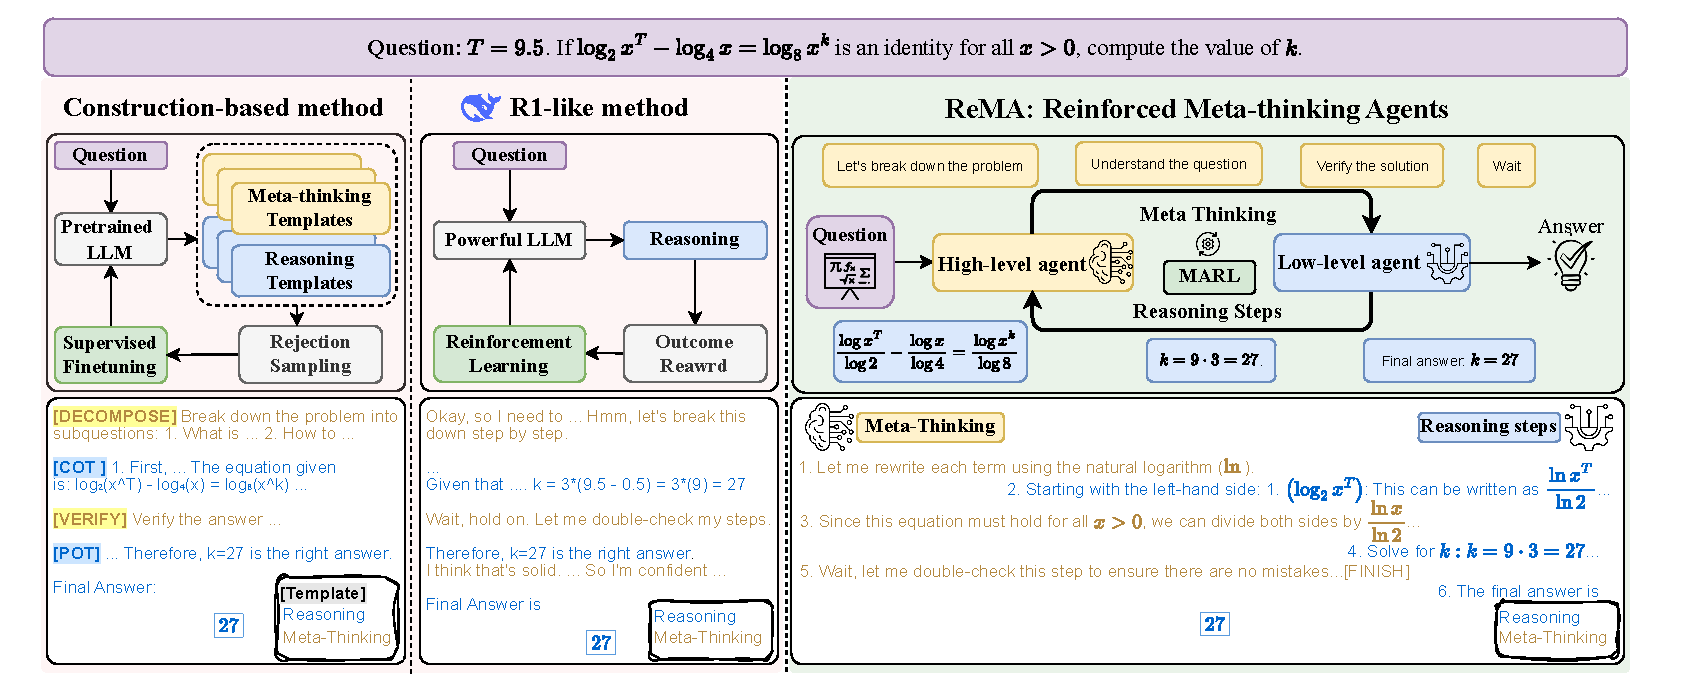
\includegraphics[width=\linewidth]{figures/mainv3/main2.pdf}
    \vspace{-10pt}
    \caption{
        Left: A construction-based method that fine-tunes LLMs using rejection sampling, searching among combinations of pre-defined templates. Middle: R1-like method learns to mix meta-thinking and detailed reasoning steps during training. Right: Our method \method~separates the meta-thinking and reasoning steps in a multi-agent system and updated by reinforcement learning.
    }
    \vspace{-10pt}
    \label{fig:main}
\end{figure}

To address these limitations, we introduce \textbf{Re}inforced \textbf{M}eta-thinking \textbf{A}gents (\method), a novel framework that leverages multi-agent reinforcement learning (MARL) to encourage LLMs to \textit{think about thinking}.
Our approach employs a multi-agent system (MAS) composed of a high-level \textbf{meta-thinking} agent, responsible for strategic oversight and instruction generation, and a low-level \textbf{reasoning} agent tasked with detailed executing processes based on provided guidance. 
We compare the inference process among the construction-based method, R1-like method, and \method~in Fig.~\ref{fig:main}.
Since MAS distributes the exploration space of SARL into multiple agents, it enables each agent to explore more structurally and efficiently during training.
Then we apply reinforcement learning on each agent with aligned reward functions. 
In this way, \method~effectively balances the trade-off between generalization capability and exploration efficiency.
As a result, they can learn to play the best of their role (either to meta-think or to follow instructions), at the present of the other agent.


To our knowledge, we are the first to formally define and optimize a multi-agent meta-thinking reasoning process (MAMRP) through multi-agent reinforcement learning.
Our extensive experiments span both math reasoning and LLM-as-a-Judge tasks, where \method~consistently achieves the highest average performance across three backbone pretrained models.
We further extend \method~to multi-turn interaction settings on math reasoning tasks, implementing turn-level ratio to optimize trajectory returns and stabilize training.
Through comprehensive ablation studies, we illustrate the evolving dynamics between agents, revealing unexpected interaction patterns such as role reversals under different reward settings.
These findings provide valuable insights into how meta-thinking processes enhance the reasoning capabilities of LLMs.

